%!TEX program = xelatex

\documentclass[11pt,titlepage]{report}
%!TEX root = main.tex

\usepackage[T1]{fontenc}
\usepackage{lmodern}
\usepackage[svgnames]{xcolor}
\usepackage{fontspec} % XeLaTeX required!
\usepackage{graphicx}
\usepackage{circuitikz}
\usepackage{tikz}
\usepackage{pifont}
\usepackage[some]{background}
\usepackage{xltxtra} 
\usepackage{setspace}
\usepackage[absolute]{textpos}
\usepackage[latin1]{inputenc}
\usepackage[english]{babel}
\usepackage{graphicx}
\usepackage{wrapfig}
\usepackage{fullpage}
\usepackage[margin=1in]{geometry}
\usepackage{float}
\usepackage{url}
\usepackage{multicol}
\usepackage{hyperref}
\usepackage{titlepic}
\usepackage{standalone}
\usepackage{siunitx}
\usepackage{booktabs}
\usepackage{amsmath}
\usepackage{unicode-math}
\usepackage{verbatim}
\usepackage{enumitem}
\usepackage{listings}
\usepackage{multirow}
\usepackage{pgfplots}
\pgfplotsset{compat=1.8}
\usepackage{caption} 
\usepackage[parfill]{parskip}
\usepackage{import}
\usepackage[backend=bibtexu,texencoding=utf8,bibencoding=utf8,style=ieee,sortlocale=en_GB,language=auto]{biblatex}
\usepackage[strict,autostyle]{csquotes}
\usepackage[final]{pdfpages}
\usepackage{subcaption}
\usepackage{ifplatform}
%\captionsetup[table]{skip=10pt}


% Fix for includepdf bug in Mac OS X
\newcommand{\insertpdfpath}[1]{
	\ifwindows
	\newcommand{\insertpdf}[2]{\includepdf[pages=##1]{##2}}
	\else
	\newcommand{\insertpdf}[2]{\includepdf[pages=##1]{#1/##2}}
	\fi
}

%set fonts
\setmainfont[Ligatures=TeX]{Myriad Pro}
\setmathfont{Asana Math}
\setmonofont{Lucida Console}

\usepackage{titlesec, color}
\renewcommand{\familydefault}{\sfdefault} %set font family
\renewcommand{\arraystretch}{1.2} %set table vertical spacing
\setlength\parindent{0pt} %no paragraph indent
\hypersetup{ %setup hyperlinks
    colorlinks,
    citecolor=black,
    filecolor=black,
    linkcolor=black,
    urlcolor=black
}

%redesign chapter headings
\definecolor{gray75}{gray}{0.75}
\newcommand{\chapternumber}{\thechapter}
\newcommand{\hsp}{\hspace{20pt}}
\titleformat{\chapter}[hang]{\Huge\bfseries}{\chapternumber\hsp\textcolor{gray75}{|}\hsp}{0pt}{\Huge\bfseries}

%Redefine appendix headers
\renewcommand{\appendixname}{Appendix}
\renewcommand{\appendixtocname}{Appendices}
\renewcommand{\appendixpagename}{Appendices}

%For code listings
\definecolor{black}{rgb}{0,0,0}
\definecolor{browntags}{rgb}{0.65,0.1,0.1}
\definecolor{bluestrings}{rgb}{0,0,1}
\definecolor{graycomments}{rgb}{0.4,0.4,0.4}
\definecolor{redkeywords}{rgb}{1,0,0}
\definecolor{bluekeywords}{rgb}{0.13,0.13,0.8}
\definecolor{greencomments}{rgb}{0,0.5,0}
\definecolor{redstrings}{rgb}{0.9,0,0}
\definecolor{purpleidentifiers}{rgb}{0.01,0,0.01}


\lstdefinestyle{csharp}{
language=[Sharp]C,
showspaces=false,
showtabs=false,
breaklines=true,
showstringspaces=false,
breakatwhitespace=true,
escapeinside={(*@}{@*)},
columns=fullflexible,
commentstyle=\color{greencomments},
keywordstyle=\color{bluekeywords}\bfseries,
stringstyle=\color{redstrings},
identifierstyle=\color{purpleidentifiers},
basicstyle=\ttfamily\small}

\lstdefinestyle{c}{
language=C,
showspaces=false,
showtabs=false,
breaklines=true,
showstringspaces=false,
breakatwhitespace=true,
escapeinside={(*@}{@*)},
columns=fullflexible,
commentstyle=\color{greencomments},
keywordstyle=\color{bluekeywords}\bfseries,
stringstyle=\color{redstrings},
identifierstyle=\color{purpleidentifiers},
}

\lstdefinestyle{matlab}{
language=Matlab,
showspaces=false,
showtabs=false,
breaklines=true,
showstringspaces=false,
breakatwhitespace=true,
escapeinside={(*@}{@*)},
columns=fullflexible,
commentstyle=\color{greencomments},
keywordstyle=\color{bluekeywords}\bfseries,
stringstyle=\color{redstrings},
identifierstyle=\color{purpleidentifiers}
}

\lstdefinestyle{vhdl}{
language=VHDL,
showspaces=false,
showtabs=false,
breaklines=true,
showstringspaces=false,
breakatwhitespace=true,
escapeinside={(*@}{@*)},
columns=fullflexible,
commentstyle=\color{greencomments},
keywordstyle=\color{bluekeywords}\bfseries,
stringstyle=\color{redstrings},
identifierstyle=\color{purpleidentifiers}
}

\lstdefinestyle{xaml}{
language=XML,
showspaces=false,
showtabs=false,
breaklines=true,
showstringspaces=false,
breakatwhitespace=true,
escapeinside={(*@}{@*)},
columns=fullflexible,
commentstyle=\color{greencomments},
keywordstyle=\color{redkeywords},
stringstyle=\color{bluestrings},
tagstyle=\color{browntags},
morestring=[b]",
  morecomment=[s]{<?}{?>},
  morekeywords={xmlns,version,typex:AsyncRecords,x:Arguments,x:Boolean,x:Byte,x:Char,x:Class,x:ClassAttributes,x:ClassModifier,x:Code,x:ConnectionId,x:Decimal,x:Double,x:FactoryMethod,x:FieldModifier,x:Int16,x:Int32,x:Int64,x:Key,x:Members,x:Name,x:Object,x:Property,x:Shared,x:Single,x:String,x:Subclass,x:SynchronousMode,x:TimeSpan,x:TypeArguments,x:Uid,x:Uri,x:XData,Grid.Column,Grid.ColumnSpan,Click,ClipToBounds,Content,DropDownOpened,FontSize,Foreground,Header,Height,HorizontalAlignment,HorizontalContentAlignment,IsCancel,IsDefault,IsEnabled,IsSelected,Margin,MinHeight,MinWidth,Padding,SnapsToDevicePixels,Target,TextWrapping,Title,VerticalAlignment,VerticalContentAlignment,Width,WindowStartupLocation,Binding,Mode,OneWay,xmlns:x}
}

\lstdefinestyle{matlab}{
language=Matlab,
showspaces=false,
showtabs=false,
breaklines=true,
showstringspaces=false,
breakatwhitespace=true,
escapeinside={(*@}{@*)},
columns=fullflexible,
commentstyle=\color{greencomments},
keywordstyle=\color{bluekeywords}\bfseries,
stringstyle=\color{purpleidentifiers},
identifierstyle=\color{purpleidentifiers}
}

%defaults
\lstset{
basicstyle=\ttfamily\small,
extendedchars=false,
numbers=left,
numberstyle=\ttfamily\tiny,
stepnumber=1,
tabsize=4,
numbersep=5pt
}
\addbibresource{../../library/bibliography.bib}

\begin{document}

\section{Labday 3}
\subsection{Report 11}
For testing purposes, we decided to transmit different signals and analyze their resulting spectra. The results are shown in Figure~\ref{fig:ass-1-rep-11}. As expected, the spectum of the \SI{2.5}{kHz} sine sampled at \SI{2}{kHz} is aliased as there are delta peaks at \SI{-2.5}{kHz} + \SI{2}{kHz} = \SI{-0.5}{kHz} and \SI{2.5}{kHz} - \SI{2}{kHz} = \SI{0.5}{kHz}. The other spectra seem just fine.

\begin{figure}[H]
	\centering
	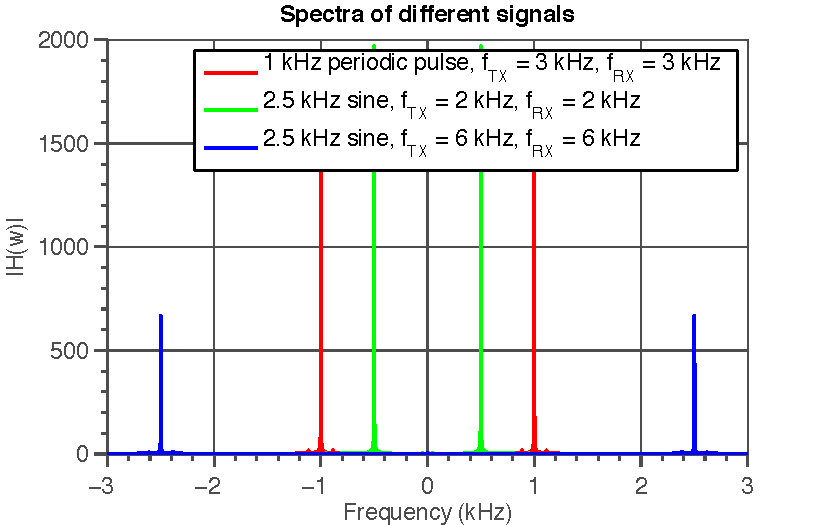
\includegraphics[width=0.6\textwidth]{../../deliverable-7-resources/figures/ass-1/report-11-12-13/ass-1-report-11-random-signals.pdf}
	\caption{Some arbitrary signal spectra, measured in the testing environment}
	\label{fig:ass-1-rep-11}
\end{figure}

Figure~\ref{fig:ass-1-rep-11-imp} shows impulse responses and their spectra samples at different frequencies. Note that there is a lot of noise in the frequencies around \SI{0}{Hz}. Let $F_{TX}$ denote the transmitting sample frequency and $F_{RX}$ the receiving sample frequency. For $F_{TX}$ \SI{22.05}{kHz} and $F_{RX}$ \SI{22.05}{kHz} we did not expect any aliasing. For $F_{TX}$ \SI{22.05}{kHz} and $F_{RX}$ \SI{8}{kHz} we did expect aliasing, as the sampling frequency is below the Nyquist frequency. For $F_{TX}$ \SI{4}{kHz} and $F_{RX}$ \SI{22.05}{kHz} we did not expect any aliasing and expect to see a highest frequency of \SI{2}{kHz}, which Figure~\ref{fig:ass-1-rep-11-imp} also shows. With $F_{RX}$ \SI{22.05}{kHz}, the highest sampling rate that can be achieved without aliasing is $F_{TX}$ \SI{22.05}{kHz}.

\begin{figure}[H]
	\centering
	\begin{subfigure}{0.49\textwidth}
		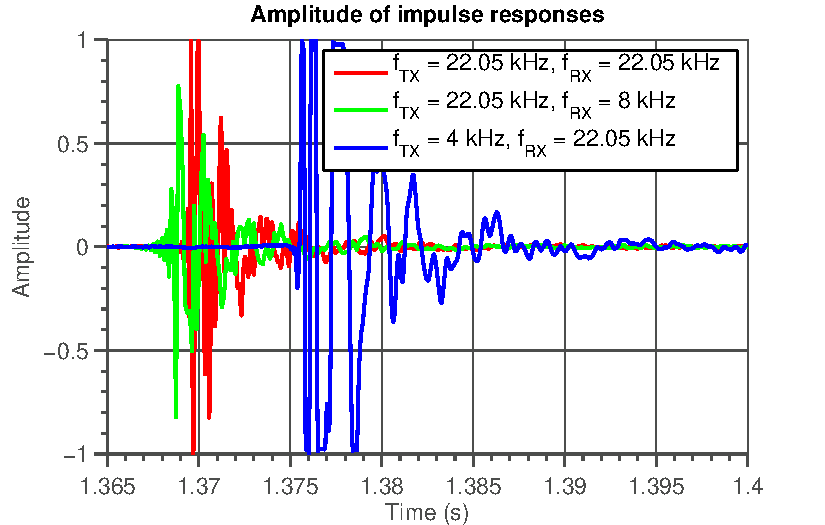
\includegraphics[width=\textwidth]{../../deliverable-7-resources/figures/ass-1/report-11-12-13/ass-1-report-11-time.pdf}
	\end{subfigure}
	\begin{subfigure}{0.49\textwidth}
		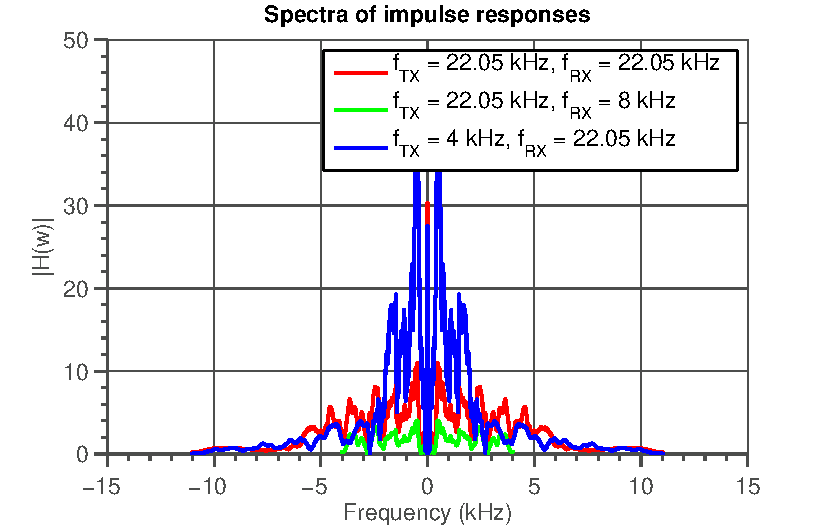
\includegraphics[width=\textwidth]{../../deliverable-7-resources/figures/ass-1/report-11-12-13/ass-1-report-11.pdf}
	\end{subfigure}
	\caption{Impulse responses and their spectra}
	\label{fig:ass-1-rep-11-imp}
\end{figure}

\subsection{Report 12}
\label{subsec:ass-1-rep-12}
As will be explained in Subsection \ref{subsec:ass-2-rep-1}, a sampling rate of \SI{34.4}{kHz} is required to obtain a spatial resolution $\Delta \lambda$ of \SI{1}{cm}.

Figure~\ref{fig:ass-1-rep-12} shows two sets of impulse responses for various distances and their delays.

\begin{figure}[H]
	\centering
	\begin{subfigure}{0.49\textwidth}
		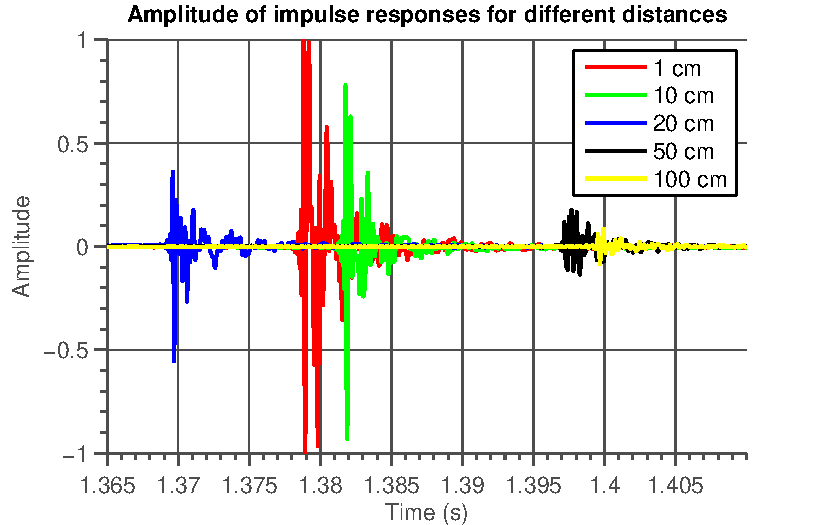
\includegraphics[width=\textwidth]{../../deliverable-7-resources/figures/ass-1/report-11-12-13/ass-1-report-13-time.pdf}
		\caption{\centering Time-domain representation of impulse responses at various distances}
	\end{subfigure}
	\begin{subfigure}{0.49\textwidth}
		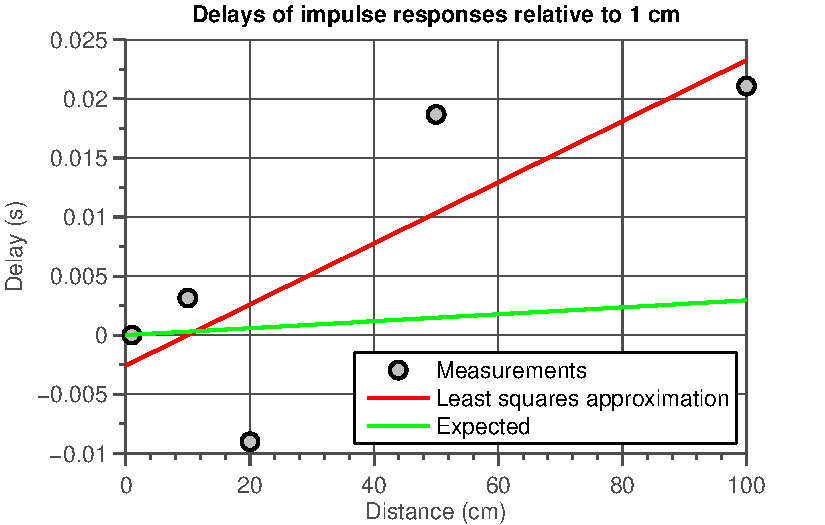
\includegraphics[width=\textwidth]{../../deliverable-7-resources/figures/ass-1/report-11-12-13/ass-1-report-13-delays.pdf}
		\caption{Delays of the impulse responses}
	\end{subfigure}
	\begin{subfigure}{0.49\textwidth}
		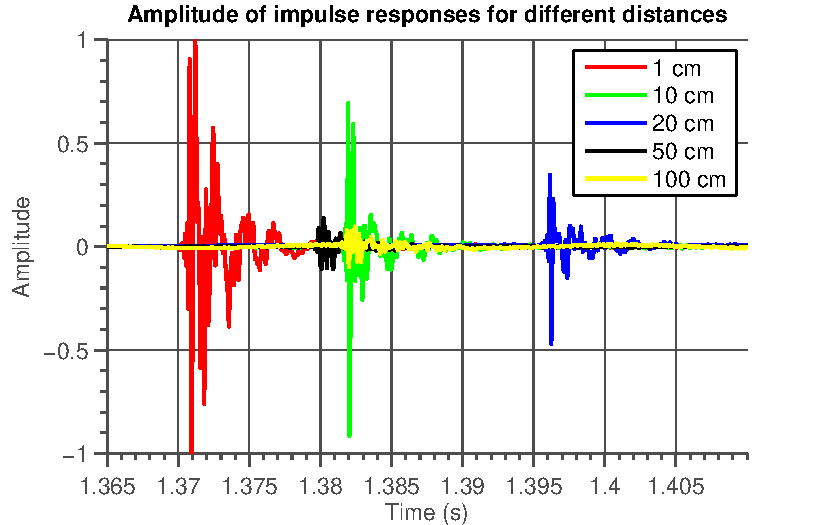
\includegraphics[width=\textwidth]{../../deliverable-7-resources/figures/ass-1/report-11-12-13/ass-1-report-13-time-set-2.pdf}
		\caption{\centering Time-domain representation of impulse responses at various distances}
	\end{subfigure}
	\begin{subfigure}{0.49\textwidth}
		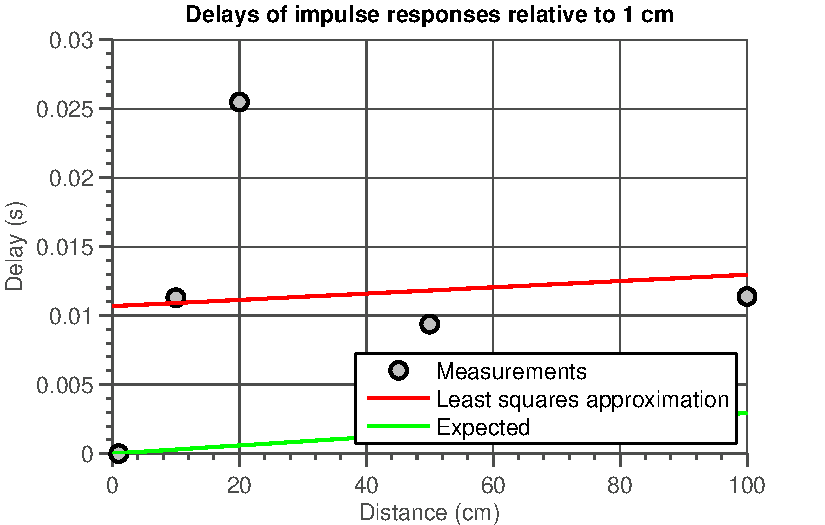
\includegraphics[width=\textwidth]{../../deliverable-7-resources/figures/ass-1/report-11-12-13/ass-1-report-13-delays-set-2.pdf}
		\caption{Delays of the impulse responses}
	\end{subfigure}
	\caption{Time plots and calculated delays of the received signal for two different measurements (set one at the top and set two at the bottom)}
	\label{fig:ass-1-rep-12}
\end{figure}

In general, we can conclude that the impulse responses are delayed and attenuated if the distance increases. This is as expected. However, their delays seem very irregular. This is due to the delays added by the signal processing software. The least squares approximations delay per unit added distance yield
\begin{align*}
	(\text{delay/unit distance added})_{\text{set one}} &= (\text{\SI{38.67}{m/s}})^{-1}, \\
	(\text{delay/unit distance added})_{\text{set two}} &= (\text{\SI{438.58}{m/s}})^{-1}.
\end{align*}
We see that these values are somewhat in the range of the speed of sound.

\subsection{Report 13}
\label{subsec:ass-1-rep-13}
The measurements of Subsection \ref{subsec:ass-1-rep-12} will now be repeated with an obstacle. Figure~\ref{fig:ass-1-rep-13-los-nlos} shows the results of these NLOS measurements.

\begin{figure}[H]
	\centering
	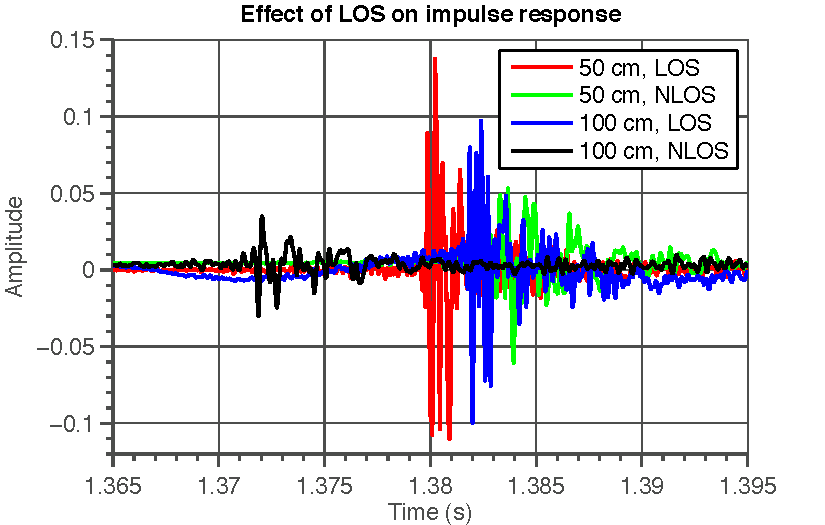
\includegraphics[width=0.6\textwidth]{../../deliverable-7-resources/figures/ass-1/report-11-12-13/ass-1-report-13-los-nlos.pdf}
	\caption{Time-domain representations of LOS and NLOS impulse responses}
	\label{fig:ass-1-rep-13-los-nlos}
\end{figure}

We see that for \SI{50}{cm} the NLOS impulse response is delayed, as expected. However, for \SI{100}{cm}, the LOS impulse response is delayed. This is probably due to measurement errors; the signal processing software introduces delays.

Because of the measurement errors, we need a reference signal to correctly measure the propagation distance. The propagation distance can still be determined in the NLOS case. However, this propagation distance will then simply correspond to a NLOS path and not be very useful.



\subsection{Report 14}
% In order to test our channel estimation we used \texttt{refsignal.m} to generate signals. The signals where send at different distances, the received signals are shown in Figure~\ref{fig:rep14-tx-rx}. From the received signals we retrieved the impulse responses which are shown in Figure~\ref{fig:rep14-impulse}. With this impulse reponses the signals send where reconstructed. The final results are shown in Figure~\ref{fig:rep14-comparison}. From this plots we can conclude the the our channel estimation works sufficiently well to be used for our TDOA localization.
Figure~\ref{fig:ass-1-rep-14-rx-tx} shows the sent and received signals by making use of the given \texttt{refsignal.m} script for various distances. Note that the amplitude is shown logaritmic to improve the readability of the graph. Figure~\ref{fig:ass-1-rep-14-imps} shows the impulse responses obtained by deconvolution by inversion.

\begin{figure}[H]
	\centering
	\begin{subfigure}{0.49\textwidth}
		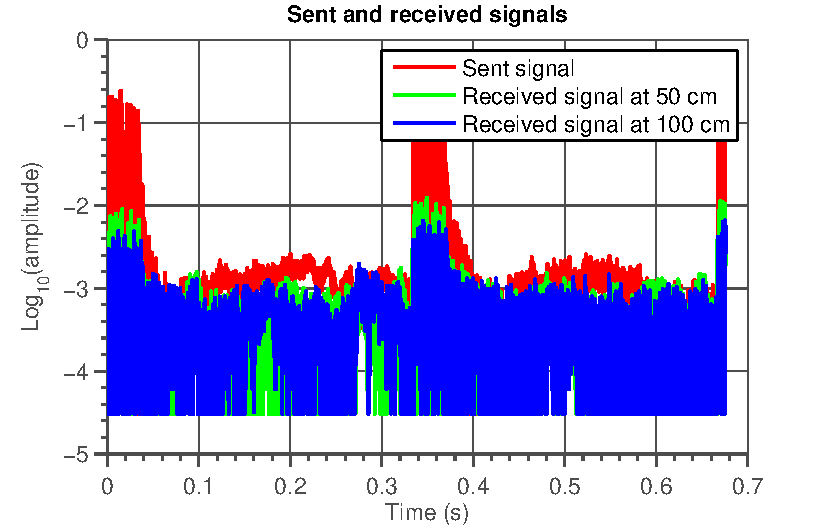
\includegraphics[width=\textwidth]{../../deliverable-7-resources/figures/ass-1/report-14-15/ass-1-report-14-sent-received.pdf}
		\caption{\centering Time-domain representation of the transmitted and received signals}
		\label{fig:ass-1-rep-14-rx-tx}
	\end{subfigure}
	\begin{subfigure}{0.49\textwidth}
		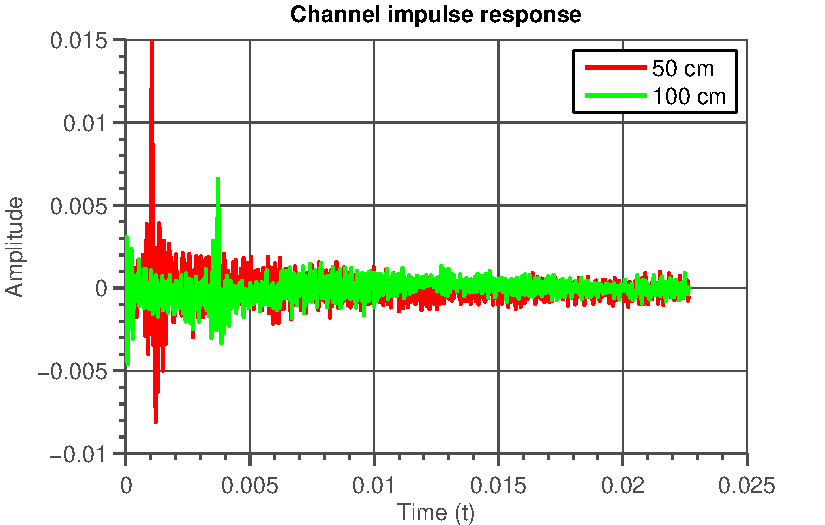
\includegraphics[width=\textwidth]{../../deliverable-7-resources/figures/ass-1/report-14-15/ass-1-report-14-impulse-responses.pdf}
		\caption{\centering Obtained channel impulse responses for the two distances}
		\label{fig:ass-1-rep-14-imps}
	\end{subfigure}
	\caption{Measurement results}
	\label{fig:ass-1-rep-14-both}
\end{figure}

We then tried to verify the obtained impulse responses by convolving the sent signal with the impulse responses. A comparison to the actual received signal can be found in Figure~\ref{fig:ass-1-rep-14-comp}.

\begin{figure}[H]
	\centering
	\begin{subfigure}{0.49\textwidth}
		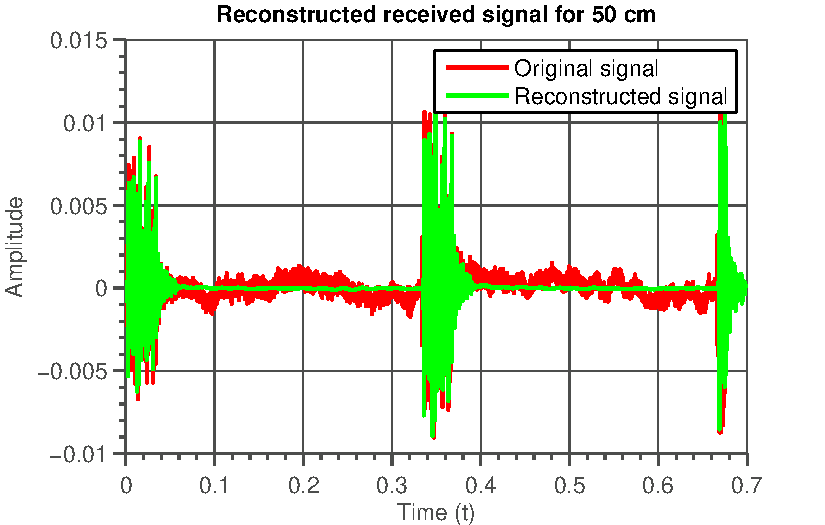
\includegraphics[width=\textwidth]{../../deliverable-7-resources/figures/ass-1/report-14-15/ass-1-report-14-50cm-reconstruction.pdf}
		\caption{\centering Reconstruction of the received signal at \SI{50}{cm}}
	\end{subfigure}
	\begin{subfigure}{0.49\textwidth}
		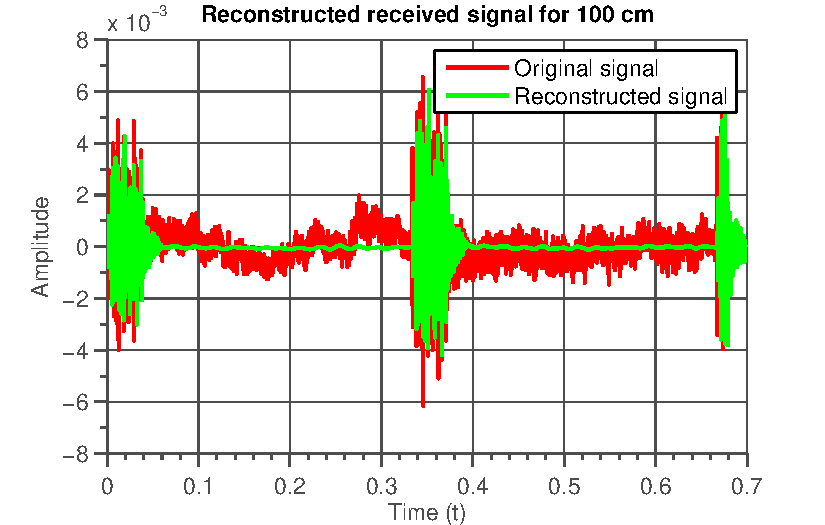
\includegraphics[width=\textwidth]{../../deliverable-7-resources/figures/ass-1/report-14-15/ass-1-report-14-100cm-reconstruction.pdf}
		\caption{\centering Reconstruction of the received signal at \SI{100}{cm}}
	\end{subfigure}
	\caption{A comparison of the received and reconstructed signal at two distances}
	\label{fig:ass-1-rep-14-comp}
\end{figure}

We see that these comparisons are a very good demonstration of the filtering property (removal of uncorrelated signals) of the deconvolution as will be explained in Subsection \ref{subsec:ass-2-rep-5}.

\subsection{Report 15}
In this report we will design the optimal parameters of the audio beacon for a maximal distance of five to six meters. For a discussion of the actual parameters chosen, see Subsection~\ref{subsec:ass-2-rep-1}. For a discussing of the properties of the sent signal of impulse response estimation, see Subsection~\ref{subsec:ass-1-rep-10}.

In the previous reports, we have seen that there is a lot noise on the lower frequencies. Therefore, we expect to use a signal at higher frequencies to increase the signal-to-noise ratio. However, due to signal processing, the signal will go most likely through audio filters. We therefore expect to use a highest frequency around \SI{20}{kHz}. To satify the Nyquist criterion, we should use the conventional \SI{44.1}{kHz} sampling frequency. This also allows for a reasonable spatial resolution $\Delta \lambda$ of \SI{0.78}{cm}.

To achieve good deconvolution properties, we will not use the theoretical sent signal, but a \SI{0}{cm} measurement. This will include filtering effects caused by signal processing and improve the performance of our algorithms.

If the properties discussed in Subsection~\ref{subsec:ass-1-rep-10} are satified, then deconvolution should result in an impulse response without a statistical significant peak.

\end{document}